\documentclass[pdftex,12pt,a4paper]{article}

\usepackage{wrapfig, amssymb, amsmath, graphicx, subfigure, tikz, float}
\usepackage[dutch]{babel}
\usepackage[top=0.5in, bottom=0.5in, left=1in, right=1in]{geometry}
\pagenumbering{arabic}
\newcommand{\HRule}{\rule{\linewidth}{0.5mm}}
\usepackage{fancyvrb}
\usepackage{color}
\usepackage[latin1]{inputenc}
\makeatletter
\def\PY@reset{\let\PY@it=\relax \let\PY@bf=\relax%
    \let\PY@ul=\relax \let\PY@tc=\relax%
    \let\PY@bc=\relax \let\PY@ff=\relax}
\def\PY@tok#1{\csname PY@tok@#1\endcsname}
\def\PY@toks#1+{\ifx\relax#1\empty\else%
    \PY@tok{#1}\expandafter\PY@toks\fi}
\def\PY@do#1{\PY@bc{\PY@tc{\PY@ul{%
    \PY@it{\PY@bf{\PY@ff{#1}}}}}}}
\def\PY#1#2{\PY@reset\PY@toks#1+\relax+\PY@do{#2}}

\expandafter\def\csname PY@tok@gd\endcsname{\def\PY@tc##1{\textcolor[rgb]{0.63,0.00,0.00}{##1}}}
\expandafter\def\csname PY@tok@gu\endcsname{\let\PY@bf=\textbf\def\PY@tc##1{\textcolor[rgb]{0.50,0.00,0.50}{##1}}}
\expandafter\def\csname PY@tok@gt\endcsname{\def\PY@tc##1{\textcolor[rgb]{0.00,0.27,0.87}{##1}}}
\expandafter\def\csname PY@tok@gs\endcsname{\let\PY@bf=\textbf}
\expandafter\def\csname PY@tok@gr\endcsname{\def\PY@tc##1{\textcolor[rgb]{1.00,0.00,0.00}{##1}}}
\expandafter\def\csname PY@tok@cm\endcsname{\let\PY@it=\textit\def\PY@tc##1{\textcolor[rgb]{0.25,0.50,0.50}{##1}}}
\expandafter\def\csname PY@tok@vg\endcsname{\def\PY@tc##1{\textcolor[rgb]{0.10,0.09,0.49}{##1}}}
\expandafter\def\csname PY@tok@m\endcsname{\def\PY@tc##1{\textcolor[rgb]{0.40,0.40,0.40}{##1}}}
\expandafter\def\csname PY@tok@mh\endcsname{\def\PY@tc##1{\textcolor[rgb]{0.40,0.40,0.40}{##1}}}
\expandafter\def\csname PY@tok@go\endcsname{\def\PY@tc##1{\textcolor[rgb]{0.53,0.53,0.53}{##1}}}
\expandafter\def\csname PY@tok@ge\endcsname{\let\PY@it=\textit}
\expandafter\def\csname PY@tok@vc\endcsname{\def\PY@tc##1{\textcolor[rgb]{0.10,0.09,0.49}{##1}}}
\expandafter\def\csname PY@tok@il\endcsname{\def\PY@tc##1{\textcolor[rgb]{0.40,0.40,0.40}{##1}}}
\expandafter\def\csname PY@tok@cs\endcsname{\let\PY@it=\textit\def\PY@tc##1{\textcolor[rgb]{0.25,0.50,0.50}{##1}}}
\expandafter\def\csname PY@tok@cp\endcsname{\def\PY@tc##1{\textcolor[rgb]{0.74,0.48,0.00}{##1}}}
\expandafter\def\csname PY@tok@gi\endcsname{\def\PY@tc##1{\textcolor[rgb]{0.00,0.63,0.00}{##1}}}
\expandafter\def\csname PY@tok@gh\endcsname{\let\PY@bf=\textbf\def\PY@tc##1{\textcolor[rgb]{0.00,0.00,0.50}{##1}}}
\expandafter\def\csname PY@tok@ni\endcsname{\let\PY@bf=\textbf\def\PY@tc##1{\textcolor[rgb]{0.60,0.60,0.60}{##1}}}
\expandafter\def\csname PY@tok@nl\endcsname{\def\PY@tc##1{\textcolor[rgb]{0.63,0.63,0.00}{##1}}}
\expandafter\def\csname PY@tok@nn\endcsname{\let\PY@bf=\textbf\def\PY@tc##1{\textcolor[rgb]{0.00,0.00,1.00}{##1}}}
\expandafter\def\csname PY@tok@no\endcsname{\def\PY@tc##1{\textcolor[rgb]{0.53,0.00,0.00}{##1}}}
\expandafter\def\csname PY@tok@na\endcsname{\def\PY@tc##1{\textcolor[rgb]{0.49,0.56,0.16}{##1}}}
\expandafter\def\csname PY@tok@nb\endcsname{\def\PY@tc##1{\textcolor[rgb]{0.00,0.50,0.00}{##1}}}
\expandafter\def\csname PY@tok@nc\endcsname{\let\PY@bf=\textbf\def\PY@tc##1{\textcolor[rgb]{0.00,0.00,1.00}{##1}}}
\expandafter\def\csname PY@tok@nd\endcsname{\def\PY@tc##1{\textcolor[rgb]{0.67,0.13,1.00}{##1}}}
\expandafter\def\csname PY@tok@ne\endcsname{\let\PY@bf=\textbf\def\PY@tc##1{\textcolor[rgb]{0.82,0.25,0.23}{##1}}}
\expandafter\def\csname PY@tok@nf\endcsname{\def\PY@tc##1{\textcolor[rgb]{0.00,0.00,1.00}{##1}}}
\expandafter\def\csname PY@tok@si\endcsname{\let\PY@bf=\textbf\def\PY@tc##1{\textcolor[rgb]{0.73,0.40,0.53}{##1}}}
\expandafter\def\csname PY@tok@s2\endcsname{\def\PY@tc##1{\textcolor[rgb]{0.73,0.13,0.13}{##1}}}
\expandafter\def\csname PY@tok@vi\endcsname{\def\PY@tc##1{\textcolor[rgb]{0.10,0.09,0.49}{##1}}}
\expandafter\def\csname PY@tok@nt\endcsname{\let\PY@bf=\textbf\def\PY@tc##1{\textcolor[rgb]{0.00,0.50,0.00}{##1}}}
\expandafter\def\csname PY@tok@nv\endcsname{\def\PY@tc##1{\textcolor[rgb]{0.10,0.09,0.49}{##1}}}
\expandafter\def\csname PY@tok@s1\endcsname{\def\PY@tc##1{\textcolor[rgb]{0.73,0.13,0.13}{##1}}}
\expandafter\def\csname PY@tok@sh\endcsname{\def\PY@tc##1{\textcolor[rgb]{0.73,0.13,0.13}{##1}}}
\expandafter\def\csname PY@tok@sc\endcsname{\def\PY@tc##1{\textcolor[rgb]{0.73,0.13,0.13}{##1}}}
\expandafter\def\csname PY@tok@sx\endcsname{\def\PY@tc##1{\textcolor[rgb]{0.00,0.50,0.00}{##1}}}
\expandafter\def\csname PY@tok@bp\endcsname{\def\PY@tc##1{\textcolor[rgb]{0.00,0.50,0.00}{##1}}}
\expandafter\def\csname PY@tok@c1\endcsname{\let\PY@it=\textit\def\PY@tc##1{\textcolor[rgb]{0.25,0.50,0.50}{##1}}}
\expandafter\def\csname PY@tok@kc\endcsname{\let\PY@bf=\textbf\def\PY@tc##1{\textcolor[rgb]{0.00,0.50,0.00}{##1}}}
\expandafter\def\csname PY@tok@c\endcsname{\let\PY@it=\textit\def\PY@tc##1{\textcolor[rgb]{0.25,0.50,0.50}{##1}}}
\expandafter\def\csname PY@tok@mf\endcsname{\def\PY@tc##1{\textcolor[rgb]{0.40,0.40,0.40}{##1}}}
\expandafter\def\csname PY@tok@err\endcsname{\def\PY@bc##1{\setlength{\fboxsep}{0pt}\fcolorbox[rgb]{1.00,0.00,0.00}{1,1,1}{\strut ##1}}}
\expandafter\def\csname PY@tok@kd\endcsname{\let\PY@bf=\textbf\def\PY@tc##1{\textcolor[rgb]{0.00,0.50,0.00}{##1}}}
\expandafter\def\csname PY@tok@ss\endcsname{\def\PY@tc##1{\textcolor[rgb]{0.10,0.09,0.49}{##1}}}
\expandafter\def\csname PY@tok@sr\endcsname{\def\PY@tc##1{\textcolor[rgb]{0.73,0.40,0.53}{##1}}}
\expandafter\def\csname PY@tok@mo\endcsname{\def\PY@tc##1{\textcolor[rgb]{0.40,0.40,0.40}{##1}}}
\expandafter\def\csname PY@tok@kn\endcsname{\let\PY@bf=\textbf\def\PY@tc##1{\textcolor[rgb]{0.00,0.50,0.00}{##1}}}
\expandafter\def\csname PY@tok@mi\endcsname{\def\PY@tc##1{\textcolor[rgb]{0.40,0.40,0.40}{##1}}}
\expandafter\def\csname PY@tok@gp\endcsname{\let\PY@bf=\textbf\def\PY@tc##1{\textcolor[rgb]{0.00,0.00,0.50}{##1}}}
\expandafter\def\csname PY@tok@o\endcsname{\def\PY@tc##1{\textcolor[rgb]{0.40,0.40,0.40}{##1}}}
\expandafter\def\csname PY@tok@kr\endcsname{\let\PY@bf=\textbf\def\PY@tc##1{\textcolor[rgb]{0.00,0.50,0.00}{##1}}}
\expandafter\def\csname PY@tok@s\endcsname{\def\PY@tc##1{\textcolor[rgb]{0.73,0.13,0.13}{##1}}}
\expandafter\def\csname PY@tok@kp\endcsname{\def\PY@tc##1{\textcolor[rgb]{0.00,0.50,0.00}{##1}}}
\expandafter\def\csname PY@tok@w\endcsname{\def\PY@tc##1{\textcolor[rgb]{0.73,0.73,0.73}{##1}}}
\expandafter\def\csname PY@tok@kt\endcsname{\def\PY@tc##1{\textcolor[rgb]{0.69,0.00,0.25}{##1}}}
\expandafter\def\csname PY@tok@ow\endcsname{\let\PY@bf=\textbf\def\PY@tc##1{\textcolor[rgb]{0.67,0.13,1.00}{##1}}}
\expandafter\def\csname PY@tok@sb\endcsname{\def\PY@tc##1{\textcolor[rgb]{0.73,0.13,0.13}{##1}}}
\expandafter\def\csname PY@tok@k\endcsname{\let\PY@bf=\textbf\def\PY@tc##1{\textcolor[rgb]{0.00,0.50,0.00}{##1}}}
\expandafter\def\csname PY@tok@se\endcsname{\let\PY@bf=\textbf\def\PY@tc##1{\textcolor[rgb]{0.73,0.40,0.13}{##1}}}
\expandafter\def\csname PY@tok@sd\endcsname{\let\PY@it=\textit\def\PY@tc##1{\textcolor[rgb]{0.73,0.13,0.13}{##1}}}

\def\PYZbs{\char`\\}
\def\PYZus{\char`\_}
\def\PYZob{\char`\{}
\def\PYZcb{\char`\}}
\def\PYZca{\char`\^}
\def\PYZam{\char`\&}
\def\PYZlt{\char`\<}
\def\PYZgt{\char`\>}
\def\PYZsh{\char`\#}
\def\PYZpc{\char`\%}
\def\PYZdl{\char`\$}
\def\PYZhy{\char`\-}
\def\PYZsq{\char`\'}
\def\PYZdq{\char`\"}
\def\PYZti{\char`\~}
% for compatibility with earlier versions
\def\PYZat{@}
\def\PYZlb{[}
\def\PYZrb{]}
\makeatother
\begin{document}
\begin{titlepage}

% Upper part of the page
\begin{flushleft}

\includegraphics[trim=23mm 0mm 0mm 0mm, width=1\textwidth]{./logo.jpg}\\[1cm] \end{flushleft}
\begin{center}
	\textsc{\Large Kansrekening en Statistiek}\\[0.5cm]

    % Title
    \HRule \\[0.4cm] { \huge \bfseries LAB-2}\\[0.4cm]

    \HRule \\[1.5cm]

    % Author and supervisor
\begin{minipage}{0.4\textwidth}
\begin{flushleft} \large \emph{Authors:}\\
Abe \textsc{Wiersma}\\
Stein \textsc{van Zwoll}\\
\end{flushleft}
\end{minipage}
\begin{minipage}{0.4\textwidth} \begin{flushright} \large \end{flushright}\end{minipage}

    \vfill

    % Bottom of the page 
    {\large \today}

\end{center}
\end{titlepage}
\pagebreak
\section{Exercise: Random Number Generators}
    \subsection{Rekenen met stochasten}
        $$E(X)=\sum\limits_{x}xP_X(x) = \sum\limits_{x}\sum\limits_{y}xP_{XY}(x,y)$$
        $$E(X) + E(Y) = \sum\limits_{x}\sum\limits_{y}xP_{XY}(x,y) + \sum\limits_{y}\sum\limits_{y}yP_{XY}(x,y) = $$
        $$\sum\limits_{x}\sum\limits_{y}(x + y)P_{XY}(x,y) = E(X+Y)$$

    \subsection{Uniform verdeelde stochasten}
        2.3 \\
        2.4 Numpy (as well as the random library) uses the Mersenne Twister pseudorandom generator. The domain of this generator is far larger than IBM's generator, so the chance of repetition is far smaller. Also, you will need far more  consecutive numbers to spot the pattern and be able to predict the further output of the generator. But it is still possible with Mersenne Twister, so if you are concerned with safety another generator should be used.\\

    \subsection{De exponentiële verdeling}
        3.1 de verwachting is $\lambda^-1$. De variantie is $\lambda^-2$\\
        3.2 $\lambda$ is de intensiteitsparameter. Met een hogere $\lambda$ zal de functie 
        met een hogere waarde beginnen, maar hij zal ook sneller afnemen. \\
        3.3 Het gemiddelde van de waarden die eruit komen zouden (ongeveer) gelijk moeten zijn aan de verwachting.
        Dus je neem het gemiddelde van de gevonden waardes en verheft die tot de macht -1.\\

\pagebreak

\section{Exercise: Betrouwbaarheids Intervallen}
    \begin{enumerate}
        \item
            Voor deze oefening is het de bedoeling een interval te bepalen uit een random selectie van 50 waarvoor het gemiddelde van de hele populatie met 95\% zekerheid binnen het interval ligt.
        \item

            $Z = \frac {\bar X-\mu}{\sigma/\sqrt{n}}$\\
            $P(-z\le Z\le z) = 1-\alpha = 0,95.$\\
            $P(Z \le z) = 1 - \frac{\alpha}2 = 0{,}975$\\
            $z = \Phi^{-1}(0.975) = 1.96$\\

            $\hat \mu=\bar X = \frac{1}{n}\sum_{i=1}^n X_i$\\
            $\text{Lower endpoint} = \bar\mu - 1.96 \frac{\sigma}{\sqrt{n}}$\\
            $\text{Upper endpoint} = \bar\mu + 1.96 \frac{\sigma}{\sqrt{n}}$
        \item
            result:
            \begin{figure}[H]
                \centering
                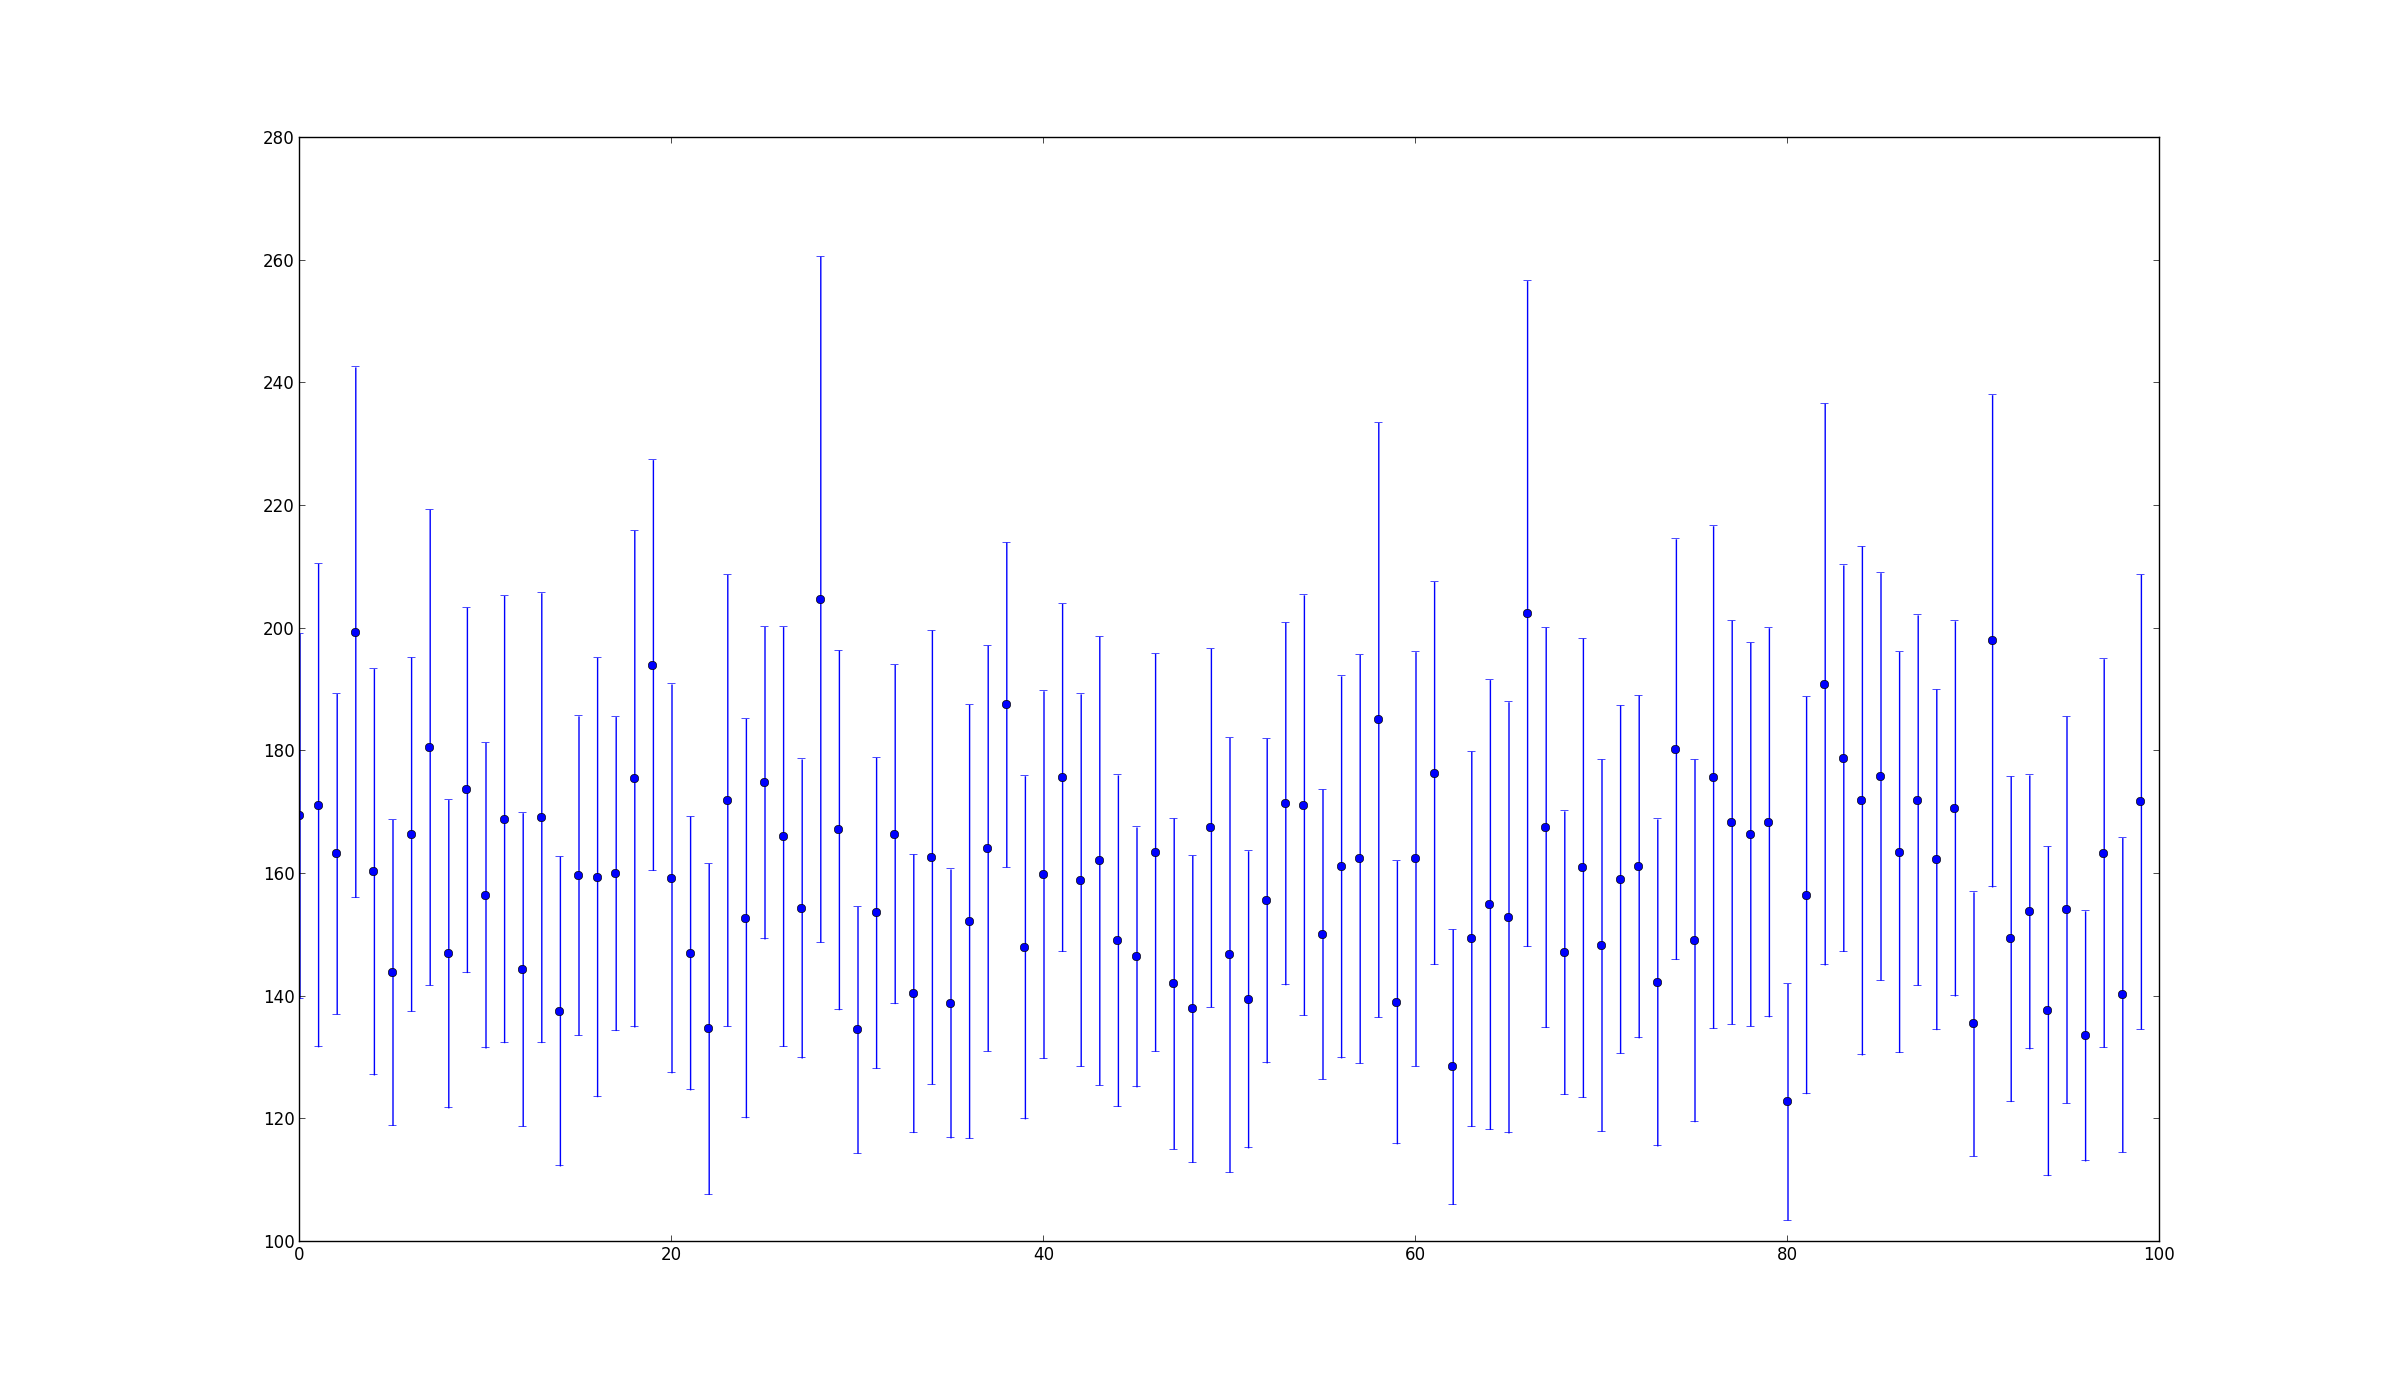
\includegraphics[width=\linewidth]{figure_1.png}
                \caption{results}
                \label{fig:results}
            \end{figure}
    \subsection{The Code}
        \begin{Verbatim}[commandchars=\\\{\}]
\PY{k+kn}{import} \PY{n+nn}{math}
\PY{k+kn}{import} \PY{n+nn}{numpy}
\PY{k+kn}{import} \PY{n+nn}{re}
\PY{k+kn}{import} \PY{n+nn}{random}
\PY{k+kn}{import} \PY{n+nn}{matplotlib.pyplot} \PY{k+kn}{as} \PY{n+nn}{plt}
\PY{k+kn}{from} \PY{n+nn}{scipy.stats} \PY{k+kn}{import} \PY{n}{norm}


\PY{k}{def} \PY{n+nf}{main}\PY{p}{(}\PY{p}{)}\PY{p}{:}
    \PY{n}{within} \PY{o}{=} \PY{l+m+mi}{0}
    \PY{n}{not\PYZus{}in} \PY{o}{=} \PY{l+m+mf}{0.05}
    \PY{n}{enddata} \PY{o}{=} \PY{p}{[}\PY{p}{]}
    \PY{n}{yerr} \PY{o}{=} \PY{p}{[}\PY{p}{]}

    \PY{c}{\PYZsh{} reading of data, with regex :)}
    \PY{n}{rawdata} \PY{o}{=} \PY{p}{[}\PY{p}{]}
    \PY{n}{ptrn} \PY{o}{=} \PY{l+s}{\PYZsq{}}\PY{l+s}{([1\PYZhy{}9][0\PYZhy{}9]*.[0\PYZhy{}9]*)\PYZdl{}}\PY{l+s}{\PYZsq{}}
    \PY{n}{lines} \PY{o}{=} \PY{p}{[}\PY{n}{line}\PY{o}{.}\PY{n}{strip}\PY{p}{(}\PY{p}{)} \PY{k}{for} \PY{n}{line} \PY{o+ow}{in} \PY{n+nb}{open}\PY{p}{(}\PY{l+s}{\PYZsq{}}\PY{l+s}{tijden\PYZhy{}medium.log}\PY{l+s}{\PYZsq{}}\PY{p}{)}\PY{p}{]}
    \PY{k}{for} \PY{n}{line} \PY{o+ow}{in} \PY{n}{lines}\PY{p}{:}
        \PY{n}{searchResult} \PY{o}{=} \PY{n}{re}\PY{o}{.}\PY{n}{search}\PY{p}{(}\PY{n}{ptrn}\PY{p}{,} \PY{n}{line}\PY{p}{)}
        \PY{k}{if} \PY{n}{searchResult}\PY{p}{:}
            \PY{k}{if} \PY{n}{searchResult}\PY{o}{.}\PY{n}{group}\PY{p}{(}\PY{l+m+mi}{1}\PY{p}{)}\PY{p}{:}
                \PY{n}{rawdata}\PY{o}{.}\PY{n}{append}\PY{p}{(}\PY{n+nb}{float}\PY{p}{(}\PY{n}{searchResult}\PY{o}{.}\PY{n}{group}\PY{p}{(}\PY{l+m+mi}{1}\PY{p}{)}\PY{p}{)}\PY{p}{)}
        \PY{k}{else}\PY{p}{:}
            \PY{k}{print} \PY{l+s}{\PYZsq{}}\PY{l+s}{line did not pass regex}\PY{l+s}{\PYZsq{}}

    \PY{k}{for} \PY{n}{pla} \PY{o+ow}{in} \PY{n+nb}{range}\PY{p}{(}\PY{l+m+mi}{100}\PY{p}{)}\PY{p}{:}
        \PY{c}{\PYZsh{} transform array to numpy array, for further numpy use.}
        \PY{n}{data} \PY{o}{=} \PY{n}{numpy}\PY{o}{.}\PY{n}{array}\PY{p}{(}\PY{n}{rawdata}\PY{p}{)}
        \PY{n}{data\PYZus{}mean} \PY{o}{=} \PY{n}{numpy}\PY{o}{.}\PY{n}{mean}\PY{p}{(}\PY{n}{data}\PY{p}{)}

        \PY{c}{\PYZsh{} draw fifty random numbers from list.}
        \PY{n}{fifty\PYZus{}random} \PY{o}{=} \PY{p}{[}\PY{p}{]}
        \PY{k}{for} \PY{n}{i} \PY{o+ow}{in} \PY{n+nb}{range}\PY{p}{(}\PY{l+m+mi}{50}\PY{p}{)}\PY{p}{:}
            \PY{n}{random\PYZus{}index} \PY{o}{=} \PY{n}{random}\PY{o}{.}\PY{n}{randrange}\PY{p}{(}\PY{n+nb}{len}\PY{p}{(}\PY{n}{data}\PY{p}{)}\PY{p}{)}
            \PY{n}{fifty\PYZus{}random}\PY{o}{.}\PY{n}{append}\PY{p}{(}\PY{n}{data}\PY{p}{[}\PY{n}{random\PYZus{}index}\PY{p}{]}\PY{p}{)}
            \PY{n}{data} \PY{o}{=} \PY{n}{numpy}\PY{o}{.}\PY{n}{delete}\PY{p}{(}\PY{n}{data}\PY{p}{,} \PY{n}{random\PYZus{}index}\PY{p}{)}

        \PY{n}{fifty\PYZus{}random} \PY{o}{=} \PY{n}{numpy}\PY{o}{.}\PY{n}{array}\PY{p}{(}\PY{n}{fifty\PYZus{}random}\PY{p}{)}

        \PY{n}{random\PYZus{}mean} \PY{o}{=} \PY{n}{numpy}\PY{o}{.}\PY{n}{mean}\PY{p}{(}\PY{n}{fifty\PYZus{}random}\PY{p}{)}
        \PY{n}{random\PYZus{}sigma} \PY{o}{=} \PY{n}{numpy}\PY{o}{.}\PY{n}{sqrt}\PY{p}{(}\PY{n}{numpy}\PY{o}{.}\PY{n}{var}\PY{p}{(}\PY{n}{fifty\PYZus{}random}\PY{p}{)}\PY{p}{)}

        \PY{c}{\PYZsh{} definition of Cumulative distributive function of x, in this case:}
        \PY{c}{\PYZsh{} 1\PYZhy{}(a/2)}
        \PY{n}{z} \PY{o}{=} \PY{n}{norm}\PY{o}{.}\PY{n}{ppf}\PY{p}{(}\PY{l+m+mf}{1.0} \PY{o}{\PYZhy{}} \PY{p}{(}\PY{l+m+mf}{0.5} \PY{o}{*} \PY{n}{not\PYZus{}in}\PY{p}{)}\PY{p}{)}
        \PY{n}{lower} \PY{o}{=} \PY{n}{random\PYZus{}mean} \PY{o}{\PYZhy{}} \PY{p}{(}\PY{n}{z} \PY{o}{*} \PY{n}{random\PYZus{}sigma} \PY{o}{/}
                               \PY{n}{numpy}\PY{o}{.}\PY{n}{sqrt}\PY{p}{(}\PY{l+m+mi}{50}\PY{p}{)}\PY{p}{)}
        \PY{n}{upper} \PY{o}{=} \PY{n}{random\PYZus{}mean} \PY{o}{+} \PY{p}{(}\PY{n}{z} \PY{o}{*} \PY{n}{random\PYZus{}sigma} \PY{o}{/}
                               \PY{n}{numpy}\PY{o}{.}\PY{n}{sqrt}\PY{p}{(}\PY{l+m+mi}{50}\PY{p}{)}\PY{p}{)}
        \PY{k}{if} \PY{n}{data\PYZus{}mean} \PY{o}{\PYZgt{}}\PY{o}{=} \PY{n}{lower} \PY{o+ow}{and} \PY{n}{data\PYZus{}mean} \PY{o}{\PYZlt{}}\PY{o}{=} \PY{n}{upper}\PY{p}{:}
            \PY{n}{within} \PY{o}{+}\PY{o}{=} \PY{l+m+mi}{1}

        \PY{n}{enddata}\PY{o}{.}\PY{n}{append}\PY{p}{(}\PY{n}{random\PYZus{}mean}\PY{p}{)}
        \PY{n}{yerr}\PY{o}{.}\PY{n}{append}\PY{p}{(}\PY{p}{[}\PY{n}{math}\PY{o}{.}\PY{n}{fabs}\PY{p}{(}\PY{n}{lower} \PY{o}{\PYZhy{}} \PY{n}{random\PYZus{}mean}\PY{p}{)}\PY{p}{,}
                     \PY{n}{math}\PY{o}{.}\PY{n}{fabs}\PY{p}{(}\PY{n}{upper} \PY{o}{\PYZhy{}} \PY{n}{random\PYZus{}mean}\PY{p}{)}\PY{p}{]}\PY{p}{)}

    \PY{n}{enddata} \PY{o}{=} \PY{n}{numpy}\PY{o}{.}\PY{n}{array}\PY{p}{(}\PY{n}{enddata}\PY{p}{)}
    \PY{n}{yerr} \PY{o}{=} \PY{n}{numpy}\PY{o}{.}\PY{n}{array}\PY{p}{(}\PY{n}{yerr}\PY{p}{)}
    \PY{n}{plt}\PY{o}{.}\PY{n}{errorbar}\PY{p}{(}\PY{n+nb}{range}\PY{p}{(}\PY{l+m+mi}{100}\PY{p}{)}\PY{p}{,} \PY{n}{enddata}\PY{p}{,} \PY{n}{yerr}\PY{o}{=}\PY{n}{yerr}\PY{o}{.}\PY{n}{T}\PY{p}{,} \PY{n}{fmt}\PY{o}{=}\PY{l+s}{\PYZsq{}}\PY{l+s}{o}\PY{l+s}{\PYZsq{}}\PY{p}{)}
    \PY{n}{plt}\PY{o}{.}\PY{n}{show}\PY{p}{(}\PY{p}{)}
    \PY{k}{print} \PY{l+s}{\PYZsq{}}\PY{l+s}{full collection mean within: }\PY{l+s}{\PYZsq{}} \PY{o}{+} \PY{n+nb}{str}\PY{p}{(}\PY{n}{within}\PY{p}{)} \PY{o}{+} \PY{l+s}{\PYZsq{}}\PY{l+s}{ of: }\PY{l+s}{\PYZsq{}} \PY{o}{+} \PY{n+nb}{str}\PY{p}{(}\PY{l+m+mi}{100}\PY{p}{)}

\PY{k}{if} \PY{n}{\PYZus{}\PYZus{}name\PYZus{}\PYZus{}} \PY{o}{==} \PY{l+s}{\PYZsq{}}\PY{l+s}{\PYZus{}\PYZus{}main\PYZus{}\PYZus{}}\PY{l+s}{\PYZsq{}}\PY{p}{:}
    \PY{n}{main}\PY{p}{(}\PY{p}{)}
        \end{Verbatim}
    \end{enumerate}
\end{document}
